\chapter{Design}

\section{Introduction to Dynamic Programming}
Dynamic Programming has many definitions, but can be summarized as method of breaking down a larger problem into sub-problems, so that if you work through the sub-problems in the right order, building each answer on the previous one, you eventually solve the larger problem.
The two attributes a problem needs to have in order to be classified as a dynamic programming problem are as follows:

\begin{definition}[Optimal Substructure]
    A problem is said to have optimal substructure if an optimal solution to the problem can be deduced from optimal solutions of some or all of its subproblems.
\end{definition}

\begin{definition}[Overlapping Subproblems]
    A problem is said to have overlapping subproblems if the problem can be broken down into subproblems which can be reused several times or a recursive algorithm would solve the same subproblem more than once resulting in repeated work. (If the subproblems do not overlap, the algorithm is categorized as a "divide and conquer" algorithm rather than a dynamic programming algorithm.)
\end{definition} 
Once we have deduced that a problem has both of these properties, we can use dynamic programming principles in order to solve the problem in an efficient manner.
When solving a dynamic programming problem, it is common to start by implementing a brute force solution which explores all subproblems and returns a solution.
We can then extend our solution to use a cache to store the results of any subproblems encountered, such that when the subproblem is encountered again we do not need to re-compute the result, instead we can simply look up the cache in constant time.
This is known as "memoization", or "top-down dynamic programming".
We can then look for any patterns in the cache table which, given an initialization (usually the base case of the recursive solution), would allow us to compute the values stored in the cache without ever traversing the decision tree of the problem itself.
This is known as "tabulation", or "bottom-up dynamic programming".
In order to demonstrate this, we will use a simple problem called The Fibonacci Problem.

\section*{The Fibonacci Problem}
\begin{description}
    \item[Problem Statement:]
        Compute $fib(n)$, the $n$'th number in the Fibonacci sequence. (Where $fib(1) = 1$, $fib(2) = 1$ and $fib(n) = fib(n-1) + fib(n-2)$.)
        
    \item[Input:] 
        A positive integer $n$.
        
    \item[Output:] 
        An positive integer $fib(n)$.
        
    \item[Example:]
        For: 

        $n = 7$
        
        $fib(n) = 13$

    \item[Explanation:]
        The Fibonacci sequence is as follows: 1,1,2,3,5,8,13,...\\
        We can see that the 7th number in the sequence is 13.

\end{description}


\subsection{Brute Force Approach to The Fibonacci Problem}

We will always start with a brute force approach, in which which will use recursion to explore all subproblems and arrive at the solution. 
We know that the base cases are $fib(1) = 1$ and $fib(2) = 1$.
By definition, we know that the recursive case is $fib(n) = fib(n-1) + fib(n-2)$.

A sample Python implementation is shown in Figure \ref{fig:fibonacci-bf}.

\begin{figure}[H]
    \centering
    \begin{lstlisting}
    def fib_bf(n):
        if n <=2: return 1
        return fib_bf(n-1) + fib_bf(n-2)
    \end{lstlisting}
    \caption{Fibonacci Brute Force Python Implementation}
    \label{fig:fibonacci-bf}
\end{figure}

In order to understand just how inefficent this approach is, consider the calculation of $fib(6)$.
Figure \ref{fig:fibonacci-bf-tree} shows the repeating subproblems, which share a color in the tree.
We can see that the amount of repeating subproblems would scale exponentially with $n$.

\begin{figure}[htbp]
    \centering
    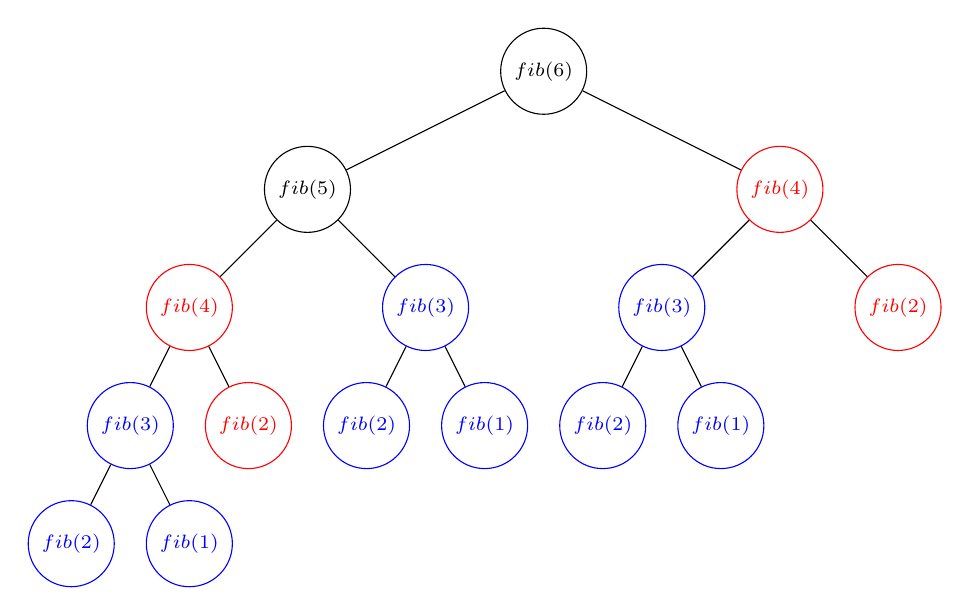
\begin{tikzpicture}[
        every node/.style={circle,draw,font=\scriptsize}, % Smaller font size
        level 1/.style={sibling distance=6cm},
        level 2/.style={sibling distance=3cm},
        level 3/.style={sibling distance=1.5cm}
    ]
        \node {$fib(6)$}
        child {node {$fib(5)$}
            child {node[red] {$fib(4)$}
                child {node[blue] {$fib(3)$}
                    child {node[blue] {$fib(2)$}}
                    child {node[blue] {$fib(1)$}}
                }
                child {node[red] {$fib(2)$}}
            }
            child {node[blue] {$fib(3)$}
                child {node[blue] {$fib(2)$}}
                child {node[blue] {$fib(1)$}}
            }
        }
        child {node[red] {$fib(4)$}
                child {node[blue] {$fib(3)$}
                    child {node[blue] {$fib(2)$}}
                    child {node[blue] {$fib(1)$}}
                }
                child {node[red] {$fib(2)$}}
            }
        ;
    \end{tikzpicture}
    
    \caption{Brute Force calculation of $fib(6) = 8$. Repeated subproblems share a color.}
    \label{fig:fibonacci-bf-tree}
\end{figure}

\subsection{Complexity Analysis of the Brute Force Approach to the Fibonacci Problem}

\begin{description}
    \item[Time Complexity:]
    At each step in the calculation of $fib(n)$, we make two 'branches', where one calculates $fib(n-1)$ and the other calculates $fib(n-2)$.
    This branching factor leads to an exponential growth in the number of function calls.
    The number of function calls grows exponentially with $n$, as each level of the tree doubles the number of function calls.
    Therefore the time complexity of this approach is $2 + 2^2 + 2^3 + ... + 2^n$ which is $O(2^n)$.
        
    \item[Space Complexity:] 
        In the brute force approach to The Fibonacci Problem, the space complexity is influenced by the recursive calls, each of which adds a frame to the call stack. However, as the recursion progresses, some of these frames can be discarded once their corresponding Fibonacci values have been computed.
        Specifically, at any point during the recursion, we only need to keep track of the previous two Fibonacci numbers. Therefore, the maximum depth of the call stack at any point is at most $n$ due to the recursion.
        This means that the space complexity of the brute force approach to compute Fibonacci numbers is $O(n)$.
        
        
    \item[Overall:] Total:\\
        Time Complexity: $O(2^n)$\\
        Space Complexity: $O(n)$
        
\end{description}
\newpage

\subsection{Memoization Approach to The Fibonacci Problem}
We can see that the optimal solution to $fib(n-1)$ + the optimal solution to $fib(n-2)$ will always be the optimal solution to $fib(n)$. This shows that the optimal substructure property holds.
We can also see that the calculation of $fib(n-1)$ contains the calculation of $fib(n-2)$, which is proof of overlapping subproblems.
This proves that The Fibonacci Problem fits the criteria for dynamic programming.
We can hence make this calculation more efficient through the use of memoization.
This simple adjustment involves storing a $(key, value)$ table called $memo$, where the key is an identifier for an intermediate subproblem and the value is the intermediate result of that subproblem.
Now, for any subproblem, we first check if the result is in $memo$ and if it is, we do not perform the calculation again, instead we return the result of that calculation from $memo$ in constant time.
If the subproblem is not in $memo$, we calculate the intermediate result and cache it in $memo$.

A sample Python implementation is shown in Figure \ref{fig:fibonacci-memo}.

\begin{figure}[H]
    \centering
    \begin{lstlisting}
    def fib_memo(n, memo={}):
        if n <= 2:
            return 1
        if n in memo:
            return memo[n]
        memo[n] = fib_memo(n-1, memo) + fib_memo(n-2, memo)
        return memo[n]
    \end{lstlisting}
    \caption{Fibonacci Memoization Python Implementation}
    \label{fig:fibonacci-memo}
\end{figure}

In the memoization solution, it is clear that we never repeat the calculation of a subproblem.
To visualize this, see Figure \ref{fig:fibonacci-memo-tree}, where repeated subproblems share a color.
We can see that we never repeat a calculation, as every time we visit a new node, we first check if it is present in $memo$, and if it is, we return the result immediately.
In this case, our $memo$ table key is $x$, and the value at $x$ returned is $fib(x)$.

\begin{figure}[H]
    \centering
    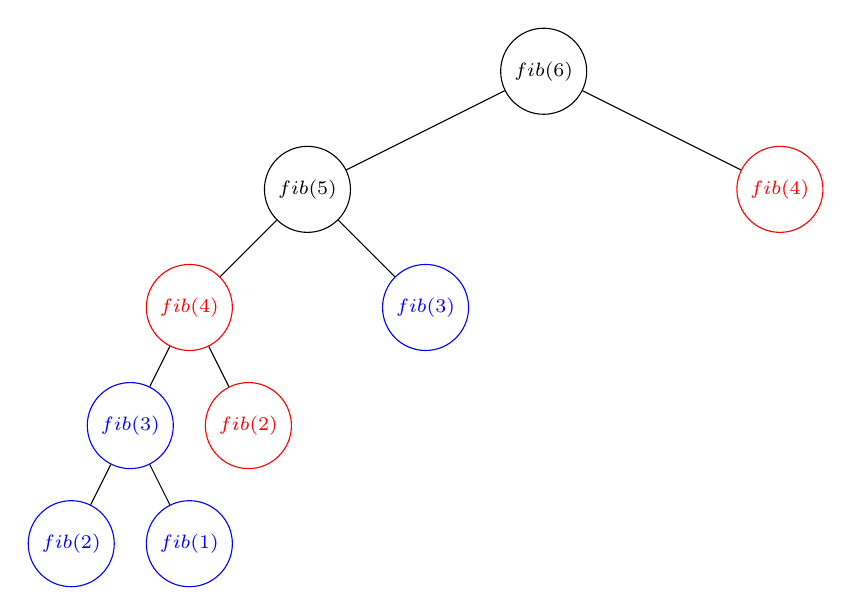
\begin{tikzpicture}[
        every node/.style={circle,draw,font=\scriptsize}, % Smaller font size
        level 1/.style={sibling distance=6cm},
        level 2/.style={sibling distance=3cm},
        level 3/.style={sibling distance=1.5cm}
    ]
        \node {$fib(6)$}
        child {node {$fib(5)$}
            child {node[red] {$fib(4)$}
                child {node[blue] {$fib(3)$}
                    child {node[blue] {$fib(2)$}}
                    child {node[blue] {$fib(1)$}}
                }
                child {node[red] {$fib(2)$}}
            }
            child {node[blue] {$fib(3)$}
            }
        }
        child {node[red] {$fib(4)$}
            }
        ;
    \end{tikzpicture}\\
    $memo$:
    \begin{table}[H]
        \centering
        \begin{tabular}{|c|c|c|c|c|c|c|}
            \hline
            \textbf{key:} & 1 & 2 & 3 & 4 & 5 & 6 \\
            \hline
            \textbf{value:} & 1 & 1 & 2 & 3 & 5 & 8 \\
            \hline
        \end{tabular}
    \end{table}
    \caption{Memoization calculation of $fib(6) = 8$. Repeated subproblems share a color.}
    \label{fig:fibonacci-memo-tree}
\end{figure}

\subsection{Complexity Analysis of the Memoization Approach to The Fibonacci Problem}

\begin{description}
    \item[Time Complexity:]
        Since each subproblem is only ever computed once, and any repeated subproblems are handled with a constant time table lookup,
        the time complexity depends only on the amount of subproblems.
        Since there are $n$ possible subproblems for any given input $n$,
        the time complexity is reduced to $O(n)$

    \item[Space Complexity:] 
        The space complexity remains determined by the recursion call stack, at $O(n)$.
        We also have to store the memo table, which contains an integer solution to each of the $n$ subproblems.
        This is also $O(n)$, giving us a total $O(2n)$ space complexity.
        This can be simplified to $O(n)$.

    \item[Overall:] Total:\\
        Time Complexity: $O(n)$\\
        Space Complexity: $O(n)$
        
\end{description}
\newpage

\subsection{Tabulation Approach to the Fibonacci Problem}
    
With the memoization approach, we saw how to compute the solution top-down, starting at $fib(n-1) + fib(n-2)$,
arriving at the base cases, and working up from there.
Notice that this step is unnecessary.
If we can deduce $fib(3)$ from $fib(2) + fib(1)$ (both of which are given in the base case),
and $fib(4)$ from $fib(3)$ and $fib(2)$,
we can work bottom-up until we arrive at $fib(n)$.
This is done by initializing an array of size $n$, placing 1 in the first and second cells as follows:
\begin{table}[H]
    \centering
    \begin{tabular}{|c|c|c|c|c|c|}
        \hline
        1 & 1 & \phantom{0} & \phantom{0} & \phantom{0} & \phantom{0} \\
        \hline
    \end{tabular}
\end{table}
And for each empty cell, filling it with the sum of the previous two cells.
This reduces the space complexity from $O(2n)$ to $O(n)$,
as all we need to do is store the table.
It is common practice to refer to the table as $dp$ in tabulation approaches.
Figure \ref{fig:fibonacci-dp-table} shows the complete $dp$ table.

\begin{figure}[H]
    \centering
    $dp$:
    \begin{table}[H]
        \centering
        \begin{tabular}{|c|c|c|c|c|c|}
            \hline
            1 & 1 & 2 & 3 & 5 & 8 \\
            \hline
        \end{tabular}
    \end{table}
    \caption{Tabulation Calculation of $fib(6)$.}
    \label{fig:fibonacci-dp-table}
\end{figure}

A sample Python implementation is shown in Figure \ref{fig:fibonacci-dp}.

\begin{figure}[H]
    \centering
    \begin{lstlisting}
    def fib_dp(n):
        if n <= 2:
            return 1

        dp = [1] * (n)

        for i in range(2, n):
            dp[i] = dp[i - 1] + dp[i - 2]

        return dp[n-1]
    \end{lstlisting}
    \caption{Fibonacci Tabulation Python Implementation}
    \label{fig:fibonacci-dp}
\end{figure}
\newpage

\subsection{Optimized Approach to the Fibonacci Problem}
We can often save space with the tabulation
approach by releasing parts of the $dp$ table which are not in use from memory.
In this case, notice that we only need $fib(n-1)$ and $fib(n-2)$ to deduce the result of $fib(n)$.
The rest of the table does not need to be stored. 
We can achieve this by storing just two variables, $prev$ and $curr$.
For an arbitrary value $x$, $curr$ represents the value of $fib(x)$, $prev$ represents the value of $fib(x-1)$.
We can calculate the result of $fib(x+1)$ from $prev$ and $curr$, then update $curr$ to the result, and $prev$ to what $curr$ was.
Starting at $curr=1$ and $prev=0$ and repeating this $n-1$ times will make $curr = fib(n)$.\\

A sample Python implementation is shown in Figure \ref{fig:fibonacci-optimized}.
\begin{figure}[H]
    \centering
    \begin{lstlisting}
    def fib_optimized(n):
        if n <= 1:
            return n
        
        prev, curr = 0, 1
        for _ in range(n-1):
            prev, curr = curr, prev + curr
            
        return curr
    \end{lstlisting}
    \caption{Fibonacci Optimized Python Implementation}
    \label{fig:fibonacci-optimized}
\end{figure}

\subsection{Complexity Analysis of the Tabulation Approach to the Fibonacci Problem}

\begin{description}
    \item[Time Complexity:]
        The time complexity remains unchanged at $O(n)$.

    \item[Space Complexity:] 
        Since we are only storing two variables of constant size at a time,
        and there is no recursion, the space complexity of this optimized version is $O(1)$.

    \item[Overall:] Total:\\
        Time Complexity: $O(n)$\\
        Space Complexity: $O(1)$
        
\end{description}
\newpage



\section{The Coin Change Problem}
\begin{description}
    \item[Problem Statement:]
        Given a list of denominations of coins $D$ and an integer amount $a$, compute the minimum amount of coins (where each coin's denomination $\in D$) needed to sum exactly to the given amount $a$.
        
    \item[Input:] 
        An integer array $D$ of possible coin denominations, and an integer amount $a$.
        
    \item[Output:] 
        An integer $r$, which represents the minimum amount of coins with denominations $\in D$ needed in order to sum exactly to $a$. If this cannot be done, return $-1$.
        
    \item[Example:]
        For: 

        $D = [1, 5, 10, 20]$

        $a = 115$

        $r = 7$

    \item[Explanation:]
        The minimum amount of coins with denominations in $D$ needed to sum to $a$ is 7.

        These coins are: $[20,20,20,20,20,10,5]$


\end{description}

The problem appears trivial at first glance. One may be tempted to use a greedy method as follows:

\subsection{Greedy Approach to the Coin Change Problem}

Algorithm~\ref{algo:coin-change-greedy} shows a greedy approach to the coin change problem.

\begin{algorithm}[H]
    \caption{Greedy Approach to the Coin Change Problem}
    \label{algo:coin-change-greedy}
    \KwIn{List of denominations of coins $D$ and an amount $a$}
    \KwOut{$r$, The minimum number of coins required to make change for $a$}
    Sort $D$ in ascending order\;
    $r \leftarrow 0$\;
    $total \leftarrow 0$\;
    \While{$\text{total} < a$}{
        \If{$|D| = 0$}{
            \KwRet{-1}\;
        }
        \If{$\text{total} + D[-1] > a$}{
            $D.\text{pop()}$\;
        }
        \Else{
            $\text{total} \leftarrow \text{total} + D[-1]$\;
            $r \leftarrow r + 1$\;
        }
    }
    \KwRet{$r$}
\end{algorithm}

In Algorithm~\ref{algo:coin-change-greedy}, we always choose the coin with the largest value which will not make the total exceed a.

\subsection{Optimality of the Greedy Approach to the Coin Change Problem}

This algorithm is not optimal, and we can prove this by counter-example.\\
A counter example is $D = [5,4,3,2,1]$, $a = 7$.\\
Given these inputs, the greedy result is: $r1 = 3$  ([5,1,1]).\\
The optimal solution for these inputs is: $r2 = 2$ ([4,3]).\\
We see that $r1 > r2$, meaning the greedy approach does not find the miminized solution.\\

\subsection{Correctness of the Greedy Approach to the Coin Change Problem}

The greedy algorithm is also not correct, and we can prove this by another counter-example.\\
A counter example is $D = [4,3]$, $a = 6$.\\
Given these inputs, the greedy result is: $r1 = -1$  ([4]).\\
The optimal solution for these inputs is: $r2 = 2$ ([3,3]).\\
We see that the greedy approach fails when a solution is indeed possible, as shown by $r2$.\\
Since we have shown that the greedy approach is neither correct nor optimal, we move on to the brute force solution.\\


\subsection{Brute Force Approach to the Coin Change Problem}

The brute force approach to the coin change problem involves generating all possible coin combinations, and checking if any of them sum exactly to $a$.
Of the ones that do, we return the minimum length.\\
To try all possible coin combinations, we can subtract each coin denomination $c \in D$ from $a$, as long as $a - c >= 0$.\\
We can repeat this step for each result obtained from this calculation (replacing $a$ with the intermediate result), until all possible coin combinations are explored.\\
We can keep track of the shortest path through the resulting tree which has a leaf value of 0, to avoid storing the entire tree in memory.\\
We return the length of the shortest path as $r$.\\


% TODO NOTE: PLOT OF ALGORITHM HERE

A sample python implementation is shown in figure \ref{fig:coin-change-bf}.

\begin{figure}[h]
    \centering
    \begin{lstlisting}
    def coin_change_bf(D, a):
        def dfs(a):
            if a == 0:
                return 0
            if a<0:
                return float('inf')
            return min([1+dfs(a-c) for c in D])
        minimum = dfs(a)
        return minimum if minimum < float("inf") else -1
    \end{lstlisting}
    \caption{Coin Change Brute Force Python Implementation}
    \label{fig:coin-change-bf}
\end{figure}

\subsection{Complexity Analysis of the Brute Force Approach to the Coin Change Problem}

\begin{description}
    \item[Time Complexity:]
    For the worst case scenario, let's assume each coin denomination $c \in D < a$ such that each node which is not a leaf node has $|D|$ children. This means we have $|D|$ recursive calls at the first level, $|D|^{2}$ at the second level, $|D|^{n}$ at the $n$'th level.\\

    The total number of recursive calls in this scenario is $|D| + |D|^{2} + ... + |D|^{a}$ which is $O(|D|^a)$.
    
    Therefore the time complexity is $O(|D|^{a})$. This is because at each step, there are $|D|$ choices (coin denominations) to consider, and the recursion depth is at most $a$ (target amount).
    
        
    \item[Space Complexity:] 
        We do not store the entire tree in memory, only the current path.

        The space complexity is determined by the maximum depth of the recursion stack. In the worst case, the recursion depth is equal to the target amount $a$. Therefore, the space complexity is $O(a)$.
        
        
    \item[Overall:] total\\
        Time Complexity: $O(|D|^a)$

        Space Complexity: $O(a)$
        
\end{description}

\subsection{Memoization Approach to the Coin Change Problem}

In the brute force algorithm, we have a chance to arrive at a value multiple times. For every path in the search tree,
we can store intermediate results in a table which we will call $memo$ (for memoization) 
so that the next time we arrive at a value, eg. 3, we don't have to repeat the work in finding the minimum amount of extra coins needed to sum to $a$.
Instead we can simply look in the table with a constant time lookup.

This optimization reduces search time greatly, as seen in subsection \ref{subsec:ca-coin-change-memo}.

A sample python implementation is shown in figure \ref{fig:coin-change-memo}.

\begin{figure}[H]
    \centering
    \begin{lstlisting}
    def coin_change_memo(D, a):
    memo = {}
    def dfs(a):
        if a == 0:
            return 0
        if a < 0:
            return float('inf')
        if a in memo:
            return memo[a]
        
        memo[a] = min([1+dfs(a-c) for c in D])
        return memo[a]
            
    res = dfs(a)
    return res if res < float("inf") else -1
    \end{lstlisting}
    \caption{Coin Change Memoization Python Implementation}
    \label{fig:coin-change-memo}
\end{figure}

\subsection{Complexity Analysis of the Memoization Approach to the Coin Change Problem}\label{subsec:ca-coin-change-memo}

\begin{description}
    \item[Time Complexity:]
    %   CITATION HERE TO THE PYTHON MANUAL
        Each unique subproblem is evaluated once, and the next time it is encountered it is retrieved from the memoization table with a constant time lookup\footnote{Python dictionary lookups have an expected $O(1)*$ time complexity.}.
        As there are $|D| * a$ unique subproblems in the worst case\footnote{$|D|$ constant time subtractions from any intermediate value $v$ where $0 \leq v \leq a$.}, the time complexity to solve all of them is $O(|D| * a)$.
    
        
    \item[Space Complexity:] 
        We need to store the $memo$ table in memory.
        The memoization table is represented by a lookup data structure where the keys range from 0 to a,
        representing the solution to each unique subproblem.
        Hence, the memory required to store the table is of order $O(a)$.
        
    \item[Overall:] total\\
        Time Complexity: $O(|D| * a)$

        Space Complexity: $O(a)$
        
\end{description}

\subsection{Tabulation Approach to the Coin Change Problem}

Instead of doing a dfs to fill in the memo table, which requires a traversal of the exponential search tree, we can calculate the values in the memo table directly, and extract the answer from there.

We will call the $memo$ table $dp$, as we are no longer doing memoization, but tabulation.

$dp[i]$ represents the minimum amount of coins needed to get the amount $i$.

For the example $D = [5,4,3,1]$, $a = 7$

We initialize each $dp[i]$ to contain infinity.

We know that $dp[0] = 0$ as it takes $0$ coins to add up to an amount of $0$. We can initialize this in our table.

Now we can deduce $dp[1], dp[2], ... dp[a]$. $dp[a]$ will contain $r$.

To get $dp[i]$, we will look at each coin $c \in D$ in sequence.

For each $c \in D$, we take $i - c$ to get $t$, and look for $dp[t]$ if it exists.

Our intermediate result is $1 + dp[t]$

If this result is less than the current $dp[i]$ and is not negative, we update $dp[i] \leftarrow 1 + dp[t]$.

The logic of this is that the amount of coins it takes to make the amount $dp[i]$ is the amount of coins it takes to make the amount $dp[t]$ plus one.

The logic is demonstrated with the examples:

Example 1: Calculating $dp[1]$\\
$dp[0]=0$\\
$dp[1]=\infty$\\
$dp[2]=\infty$\\
$dp[3]=\infty$\\
$dp[4]=\infty$\\
$dp[5]=\infty$\\
$dp[6]=\infty$\\

To calculate $dp[1]$:

For $c \in D = [5,4,3,1]$

$t = i-c = 1-5 = -4$, ignore because negative

$t = i-c = 1-4 = -3$, ignore because negative

$t = i-c = 1-3 = -2$, ignore because negative

$t = i-c = 1-1 = 0$

Look up the value of $dp[t] = 0$.

Now we take $1 + dp[0] = 1$.

This means a possible solution to $dp[1]$ is 1.

Since $1 < \infty$, we update $dp[1] \rightarrow 1$

Example 2: Calculating $dp[7]$\\
$dp[0]=0$\\
$dp[1]=1$\\
$dp[2]=2$\\
$dp[3]=1$\\
$dp[4]=1$\\
$dp[5]=1$\\
$dp[6]=2$\\
$dp[7]=\infty$\\

To calculate $dp[7]$:

For each $c \in D = [5,4,3,1]$:

$t = i-c = 7-5 = 2$, $dp[2] = 2$, $1 + dp[2] = 3$, $3 < \infty$, update $dp[7] \rightarrow 3$

$t = i-c = 7-4 = 3$, $dp[3] = 1$, $1+dp[3] = 2$, $2 < 3$, update $dp[7] \rightarrow 2$

$t = i-c = 7-3 = 4$, $dp[4] = 1$, $1+dp[4] = 2$, $2 = 2$, ignore

$t = i-c = 7-1 = 6$, $dp[6] = 2$, $1+dp[6] = 3$, $3 > 2$, ignore

We conclude that the minimum solution to $dp[7] is 2$, achieved by adding a 4 coin to $dp[3]$, which is achieved by adding a 3 coin to $dp[0]$

A sample python implementation is shown in figure \ref{fig:coin-change-dp}.

\begin{figure}[H]
    \centering
    \begin{lstlisting}
    def coin_change_dp(D,a):
        dp=[float('inf')] * (a + 1)
        dp[0] = 0
    
        for i in range(1, a+1):
            for c in D:
                t = i - c
                if t >= 0:
                    dp[i] = min(dp[i], 1+dp[t])
    
        return dp[a] if dp[a] != float('inf') else -1
    \end{lstlisting}
    \caption{Coin Change Tabulation Python Implementation}
    \label{fig:coin-change-dp}
\end{figure}

\subsection{Complexity Analysis of the Tabulation Approach to the Coin Change Problem}

\begin{description}
    \item[Time Complexity:]
        % REFERENCE TO PYTHON MANUAL
        For the worst case scenario, we need to iterate for all $i = 0; i <= a; i++$.
        And for each $i$, we need to iterate over each coin $c \in D$.
        All other operations within the loops are constant time lookups and subtractions, so the time complexity is $O(|D| * a)$
            
    \item[Space Complexity:] 
        The space complexity is determined by the size of the $dp$ array. This array is always of size $a+1$.
        Therefore the space complexity is $O(a)$
        
    \item[Overall:] Total:\\
        Time Complexity: $O(|D| * a)$

        Space Complexity: $O(a)$
        
\end{description}

\section{Longest Increasing Subsequence}

\begin{description}
    \item[Problem Statement:]
        Given an array, return the length of the longest strictly increasing subsequence in the array.
        A sequence is said to be increasing if and only if \\$x1<x2<x3<...xn$.
        A subsequence does not have to be contiguous.

    \item[Input:]
        An integer array $nums$.
        
    \item[Output:]
        An integer $lis(nums)$, the length of the longest increasing subsequence of $nums$.
    \item[Example:] For:\\
        $nums = [2,5,3,7,101,18]$\\
        $lis(nums) = 4$

    \item[Explanation:]
    The subsequence $[2,5,7,101]$ is the longest increasing subsequence in $nums$, and has length $4$.

        
\end{description}

Much like coin change, this problem appears trivial at first glance. One may attempt to be greedy as follows:

\subsection{Greedy Approach to Longest Increasing Subsequence}

\begin{algorithm}
    \caption{Greedy Approach to Longest Increasing Subsequence}
    \label{algo:lis-greedy}
    \KwIn{An integer array $nums$.}
    \KwOut{An integer $lis$, the longest increasing subsequence in $nums$.}
    $lis \leftarrow 0$\;
    $index \leftarrow 0$\;
    $cur \leftarrow nums[0]$\;
    \While{$index \leq |nums|$}{
        \If{$nums[index] > cur$}{
            $lis += 1$\;
            $cur \leftarrow nums[index]$\;
        }
        $index +=1$\;
    }
    \KwRet{$lis$}
\end{algorithm}
In Algorithm \ref{algo:lis-greedy} we iterate through nums keeping track of the current max value enountered, incrementing our result each time a new larger value is encountered.

\subsection{Optimality of the Greedy Approach to Longest Increasing Subsequence}

This algorithm is not optimal however, and we can prove this by counter-example.
Take:$$nums = [10,9,2,5,3,7,101,18]$$
Given these inputs, the greedy result is: $r1 = 2  ([10,101])$.\\
An optimal solution for these inputs is: $r2 = 4 ([2,3,7,101])$.\\
We see that $r1 > r2$, meaning the greedy approach does not find the maximised solution.
We therefore need a more sophisticated approach.

\subsection{Brute Force Approach to Longest Increasing Subsequence}

We can try a brute force approach, where we start at $nums[0]$, and for each $i \in nums$ we generate two subsequences,
one where we  exclude $i$ from the subsequence and one where we include $i$ in the subsequence if
$nums[current\_index] > nums[prev\_index]$ (So that we ensure each subsequence generated is strictly increasing).
We keep track of the $prev\_index$, which represents the last index we included in the result,
and the $current\_index$, which is the index for which we are making the choice.
This will generate all possible increasing subsequenes.
We keep track of the length of the longest increasing subsequence, and return it once all increasing subsequences are explored.

A sample Python implementation is shown in Figure \ref{fig:lis-bf}.

\begin{figure}[H]
    \centering
    \begin{lstlisting}
    def lis_bf(nums):
        def dfs(prev_index, current_index):
            # Base case: reached the end of the sequence
            if current_index == len(nums):
                return 0
            # Case 1: Exclude the current element
            exclude_current = dfs(prev_index, current_index + 1)
            # Case 2: Include the current element if it is greater than the previous one
            include_current = 0
            if prev_index < 0 or nums[current_index] > nums[prev_index]:
                include_current = 1 + dfs(current_index, current_index + 1)
            # Return the maximum length of the two cases
            return max(exclude_current, include_current)
        # Start the recursion with initial indices (-1 represents no previous index)
        return dfs(-1, 0)
    \end{lstlisting}
    \caption{Longest Increasing Subsequence Brute Force Python Implementation}
    \label{fig:lis-bf}
\end{figure}

\subsection{Complexity Analysis of the Brute Force Approach to Longest Increasing Subsequence}
Let $n$ be the length of $nums$.
\begin{description}
    \item[Time Complexity:]
        For the worst case scenario, there are $n$ indices to consider.
        There are two subtrees at each decision, one where we include the current index, and one where we do not.
        This brings the time complexity to $O(2^n)$.
        
    \item[Space Complexity:] 
        The space complexity is determined by the recursion depth,
        as once we explore a path in the recursion tree, we can release it from memory when we go to the next path.
        Therefore the space complexity is $O(n)$.
        
        
    \item[Overall:] Total:\\
        Time Complexity: $O(2^n)$\\
        Space Complexity: $O(n)$
        

\end{description}


\subsection{Memoization Approach to Longest Increasing Subsequence}

Note that for an aribitrary longest increasing subsequence of length $k$ ending at index $i$,
if there exists exactly one number which can extend the sequence, the length of the total subsequence is guaranteed to be $k+1$.
This shows the optimal substructure property.
Also, when looking for subsequences at index $i$,
we must re-compute all of the subsequences at index $i-1$.
This shows the overlapping subproblems property.
We can use memoization to avoid repeating subproblems, such as when we are deciding wether the next element should be added or not for multiple subsequences ending in the same element.
The memoization approach goes as follows:
We initialize an empty dictionary called $memo$,
the keys of which are constructed by making a tuple of $(prev\_index, current\_index)$.
Before proceeding with the recursive calls, the function checks if the result for the current combination of $prev\_index$ and $current\_index$ is already computed and stored in the $memo$ dictionary.
If it is, the stored result is returned immediately.
This optimization allows the algorithm to avoid repeating work,
speeding up the runtime significantly.
Notice that memoization is not a space efficient approach to solving subsequence problems, as there is usually a lot of subproblems to store. In the case of longest increasing subsequence, memoization actually has a worse space complexity than the brute force approach.

A sample python implementation is shown in Figure \ref{fig:lis-memo}.

\begin{figure}[H]
    \centering
    \begin{lstlisting}
    def lis_memo(nums):
        if not nums:
            return 0
    
        memo = {}
    
        def dfs(prev_index, current_index):
            if current_index == len(nums):
                return 0
    
            if (prev_index, current_index) in memo:
                return memo[(prev_index, current_index)]
            
            exclude_current = dfs(prev_index, current_index + 1)
    
            include_current = 0
            if prev_index < 0 or nums[current_index] > nums[prev_index]:
                include_current = 1 + dfs(current_index, current_index + 1)
    
            memo[(prev_index, current_index)] = max(include_current, exclude_current)
    
            return memo[(prev_index, current_index)]
    
        return dfs(-1, 0)
    \end{lstlisting}
    \caption{Longest Increasing Subsequence Memoization Python Implementation}
    \label{fig:lis-memo}
\end{figure}

\subsection{Complexity Analysis of the Memoization Approach to Longest Increasing Subsequence}
Let n be the length of nums.
\begin{description}
    \item[Time Complexity:]
        For each unique combination of $(prev\_index, current\_index)$, the algorithm either calculates the result or looks it up in the $memo$ table.
        Each subproblem is calculated only once.
        The algorithm explores all combinations of $prev\_index$ and $current\_index$.
        There are at most $n$ choices for $current\_index$ and,
        in the worst case, $n$ choices for $prev\_index$ for each $current\_index$.
        Therefore, the total number of unique subproblems is $O(n^2)$.
        
    \item[Space Complexity:] 
        The space complexity is increased to $O(n^2)$,
        as the $memo$ table needs to store all $n^2$ combinations of $prev\_index$ and $current\_index$ in the worst case.
        
        
    \item[Overall:] Total:\\
        Time Complexity: $O(n^2)$\\
        Space Complexity: $O(n^2)$
    
\end{description}

\subsection{Tabulation Approach to Longest Increasing Subsequence}
We can use tabulation to build a table from which we can deduce the result, similar to the Coin Change Problem.
We know that a subsequence which consists of only the last index will result in an increasing subsequence of length 1.
We can work backwards, for the second last, third last ect.. deciding if including that element will result in a longer increasing subsequence or not,
and storing the longest possible increasing subsequence starting at each index until we reach index 0.
We create a table called $dp$ of size $|nums|$, where $dp[i]$ represents the longest increasing subsequence starting at index $i$ in nums.
Lets take the following example:$$nums = [1,2,4,3]$$
We initialize $dp[3] \leftarrow 1$, as the longest increasing subsequence starting at index 3 is 1.
\begin{table}[H]
    \centering
    $dp:$
    \begin{tabular}{|c|c|c|c|}
        \hline
        \phantom{0} & \phantom{0} & \phantom{0} & 1 \\
        \hline
    \end{tabular}
\end{table}
Now, consider $nums[2] = 4$
We can either take $nums[2]$ as a subsequence by itself, or include $nums[2]$ in any subsequence at any index that comes after it (as long as it maintains the property of an increasing subsequence).
Including it would make $dp[2] = 1+dp[3]$,
Excluding it would make $dp[2] = 1$.
Since including it would not result in an increasing subsequence, we must exclude it, so $dp[2] = 1$.
\begin{table}[H]
    \centering
    $dp:$
    \begin{tabular}{|c|c|c|c|}
        \hline
        \phantom{0} & \phantom{0} & 1 & 1 \\
        \hline
    \end{tabular}
\end{table}
Now Conisder $nums[1] = 2$.
We can either take it by itself or include it in any subsequence at any index that comes after it and maintains the increasing subsequence property.
Including it would make $dp[1] = max(1+dp[2], 1+dp[3])$, and taking it by itself would make $dp[1] = 1$.
We choose the option which maximizes the value of $dp[1]$, which is $1+dp[2]$ (or, equally, $1+dp[3]$) $= 2$.
\begin{table}[H]
    \centering
    $dp:$
    \begin{tabular}{|c|c|c|c|}
        \hline
        \phantom{0} & 2 & 1 & 1 \\
        \hline
    \end{tabular}
\end{table}
To generalize this, we set each $dp[i]$ to $max(1,1+dp[j1],1+dp[j2],1+dp[j3]...)$ where $jx$ is the index which comes $x$ places after $i$.
We only include $1+dp[jx]$ in the max function if $nums[i] < nums[jx]$, to maintain increasing subsequence property.
This will give us a table where $dp[i]$ contains the longest increasing subsequence of $nums$ where the first number is $nums[i]$.
We can then simply return $max(dp)$.\\

A sample python implementation is shown in Figure \ref{fig:lis-dp}.

\begin{figure}[H]
    \centering
    \begin{lstlisting}
    def lis_dp(nums):
        dp = [1] * len(nums)
    
        for i in range(len(nums)-1,-1,-1):
            for j in range(i+1,len(nums)):
                if nums[i] < nums[j]:
                    dp[i] = max(dp[i], 1+dp[j])
    
        return max(dp)
    \end{lstlisting}
    \caption{Longest Increasing Subsequence Tabulation Python Implementation}
    \label{fig:lis-dp}
\end{figure}

\subsection{Complexity Analysis of the Tabulation Approach to Longest Increasing Subsequence}
Let n be the length of nums.
\begin{description}
    \item[Time Complexity:]
        For the worst case scenario, we need to perform a double nested iteration over nums.
        All other operations within the loops are constant time, so the time complexity is of order $O(n^2)$.
        
    \item[Space Complexity:] 
        The space complexity is determined by the size of the $dp$ array. This array is always of size $n$.
        Therefore the space complexity is $O(n)$.
        
        
    \item[Overall:] Total:\\
        Time Complexity: $O(n^2)$\\
        Space Complexity: $O(n)$
    
\end{description}
